
 \documentclass[12 pt]{article}\usepackage[]{graphicx}\usepackage[]{color}
%% maxwidth is the original width if it is less than linewidth
%% otherwise use linewidth (to make sure the graphics do not exceed the margin)
\makeatletter
\def\maxwidth{ %
  \ifdim\Gin@nat@width>\linewidth
    \linewidth
  \else
    \Gin@nat@width
  \fi
}
\makeatother

\definecolor{fgcolor}{rgb}{0.345, 0.345, 0.345}
\newcommand{\hlnum}[1]{\textcolor[rgb]{0.686,0.059,0.569}{#1}}%
\newcommand{\hlstr}[1]{\textcolor[rgb]{0.192,0.494,0.8}{#1}}%
\newcommand{\hlcom}[1]{\textcolor[rgb]{0.678,0.584,0.686}{\textit{#1}}}%
\newcommand{\hlopt}[1]{\textcolor[rgb]{0,0,0}{#1}}%
\newcommand{\hlstd}[1]{\textcolor[rgb]{0.345,0.345,0.345}{#1}}%
\newcommand{\hlkwa}[1]{\textcolor[rgb]{0.161,0.373,0.58}{\textbf{#1}}}%
\newcommand{\hlkwb}[1]{\textcolor[rgb]{0.69,0.353,0.396}{#1}}%
\newcommand{\hlkwc}[1]{\textcolor[rgb]{0.333,0.667,0.333}{#1}}%
\newcommand{\hlkwd}[1]{\textcolor[rgb]{0.737,0.353,0.396}{\textbf{#1}}}%

\usepackage{framed}
\makeatletter
\newenvironment{kframe}{%
 \def\at@end@of@kframe{}%
 \ifinner\ifhmode%
  \def\at@end@of@kframe{\end{minipage}}%
  \begin{minipage}{\columnwidth}%
 \fi\fi%
 \def\FrameCommand##1{\hskip\@totalleftmargin \hskip-\fboxsep
 \colorbox{shadecolor}{##1}\hskip-\fboxsep
     % There is no \\@totalrightmargin, so:
     \hskip-\linewidth \hskip-\@totalleftmargin \hskip\columnwidth}%
 \MakeFramed {\advance\hsize-\width
   \@totalleftmargin\z@ \linewidth\hsize
   \@setminipage}}%
 {\par\unskip\endMakeFramed%
 \at@end@of@kframe}
\makeatother

\definecolor{shadecolor}{rgb}{.97, .97, .97}
\definecolor{messagecolor}{rgb}{0, 0, 0}
\definecolor{warningcolor}{rgb}{1, 0, 1}
\definecolor{errorcolor}{rgb}{1, 0, 0}
\newenvironment{knitrout}{}{} % an empty environment to be redefined in TeX

\usepackage{alltt}

\usepackage{amsmath}  % Better maths support
 \usepackage{setspace}
 \usepackage{txfonts}
 \usepackage{soul}
 \usepackage[left=1 in,top=1 in,right=1 in]{geometry}
\doublespacing
\setlength{\parindent}{0.5 in}


\title {POL SCI 231b:  Section 7}
\author{GSI Guadalupe Tu\~n\'on\\University of California, Berkeley\\Spring 2016\\ ~\\ }
\date{}
\IfFileExists{upquote.sty}{\usepackage{upquote}}{}
\begin{document}

\maketitle
% Generates a title based on the \title, \author, and \date commands in the preamble.

\singlespacing




\section*{Today}
\begin{enumerate}
\item Variance of the Difference in Differences estimator
\item Randomization inference with covariates
\item Clustering
\item OLS vs fGLS - Huber-White SEs
\end{enumerate}


\clearpage
\section*{Variance of the Difference in Differences estimator}

\subsection*{A DGP (building losely from Miguel et. al).}

\begin{knitrout}
\definecolor{shadecolor}{rgb}{0.969, 0.969, 0.969}\color{fgcolor}\begin{kframe}
\begin{alltt}
\hlcom{# Pre-treatment covariates}
\hlstd{conflict_pre} \hlkwb{<-} \hlkwd{rnorm}\hlstd{(}\hlnum{100}\hlstd{,} \hlnum{95}\hlstd{,} \hlnum{4}\hlstd{)}
\hlstd{rural} \hlkwb{<-} \hlkwd{rbinom}\hlstd{(}\hlnum{100}\hlstd{,} \hlnum{1}\hlstd{,} \hlnum{0.7}\hlstd{)}
\hlstd{ethnic_frac} \hlkwb{<-} \hlkwd{rnorm}\hlstd{(}\hlnum{100}\hlstd{,} \hlnum{0.45}\hlstd{,} \hlnum{0.3}\hlstd{)}

\hlcom{# Potential outcomes}
\hlstd{y_i0} \hlkwb{<-} \hlnum{2.5} \hlopt{*} \hlstd{conflict_pre} \hlopt{+} \hlkwd{runif}\hlstd{(}\hlnum{100}\hlstd{)}
\hlstd{y_i1} \hlkwb{<-} \hlstd{y_i0} \hlopt{-} \hlkwd{rnorm}\hlstd{(}\hlnum{100}\hlstd{,} \hlnum{10}\hlstd{,} \hlnum{5}\hlstd{)} \hlopt{+} \hlkwd{rnorm}\hlstd{(}\hlnum{100}\hlstd{,}
    \hlnum{4} \hlopt{*} \hlstd{ethnic_frac,} \hlnum{3}\hlstd{)} \hlopt{-} \hlnum{8} \hlopt{*} \hlstd{rural}
\end{alltt}
\end{kframe}
\end{knitrout}

\begin{knitrout}
\definecolor{shadecolor}{rgb}{0.969, 0.969, 0.969}\color{fgcolor}\begin{kframe}
\begin{alltt}
\hlkwd{par}\hlstd{(}\hlkwc{mfrow} \hlstd{=} \hlkwd{c}\hlstd{(}\hlnum{1}\hlstd{,} \hlnum{3}\hlstd{))}
\hlkwd{plot}\hlstd{(conflict_pre, y_i1,} \hlkwc{pch} \hlstd{=} \hlnum{16}\hlstd{,} \hlkwc{col} \hlstd{=} \hlstr{"springgreen4"}\hlstd{)}
\hlkwd{plot}\hlstd{(conflict_pre, y_i0,} \hlkwc{pch} \hlstd{=} \hlnum{16}\hlstd{,} \hlkwc{col} \hlstd{=} \hlstr{"springgreen4"}\hlstd{)}
\hlkwd{plot}\hlstd{(y_i0, y_i1,} \hlkwc{pch} \hlstd{=} \hlnum{16}\hlstd{,} \hlkwc{col} \hlstd{=} \hlstr{"springgreen4"}\hlstd{)}
\end{alltt}
\end{kframe}

{\centering 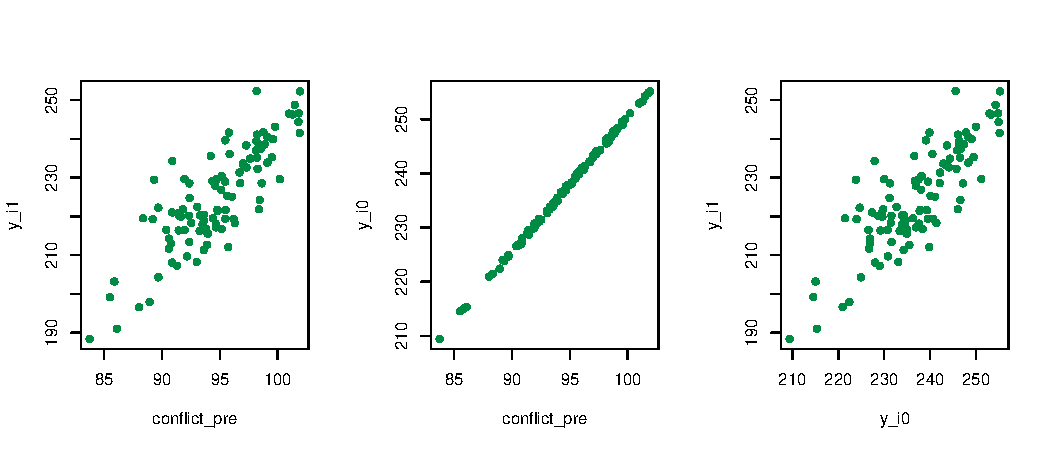
\includegraphics[width=\maxwidth]{figure/minimal-unnamed-chunk-2-1} 

}



\end{knitrout}

\begin{knitrout}
\definecolor{shadecolor}{rgb}{0.969, 0.969, 0.969}\color{fgcolor}\begin{kframe}
\begin{alltt}
\hlstd{true_ace} \hlkwb{<-} \hlkwd{mean}\hlstd{(y_i1)} \hlopt{-} \hlkwd{mean}\hlstd{(y_i0)}
\hlstd{true_ace}
\end{alltt}
\begin{verbatim}
## [1] -12.25455
\end{verbatim}
\end{kframe}
\end{knitrout}

\subsection*{A simulation}
\begin{knitrout}
\definecolor{shadecolor}{rgb}{0.969, 0.969, 0.969}\color{fgcolor}\begin{kframe}
\begin{alltt}
\hlstd{experiment} \hlkwb{<-} \hlkwa{function}\hlstd{() \{}

    \hlstd{rainfall} \hlkwb{<-} \hlkwd{rbinom}\hlstd{(}\hlnum{100}\hlstd{,} \hlnum{1}\hlstd{,} \hlnum{0.5}\hlstd{)}
    \hlstd{observed_conflict} \hlkwb{<-} \hlkwd{ifelse}\hlstd{(rainfall} \hlopt{==} \hlnum{1}\hlstd{,}
        \hlstd{y_i1, y_i0)}

    \hlcom{# simple difference of means}
    \hlstd{DM} \hlkwb{<-} \hlkwd{mean}\hlstd{(observed_conflict[rainfall} \hlopt{==} \hlnum{1}\hlstd{])} \hlopt{-}
        \hlkwd{mean}\hlstd{(observed_conflict[rainfall} \hlopt{==} \hlnum{0}\hlstd{])}

    \hlcom{# rescaling outcome (difference in}
    \hlcom{# differences)}
    \hlstd{rescaled} \hlkwb{<-} \hlstd{observed_conflict} \hlopt{-} \hlstd{conflict_pre}
    \hlstd{DiD} \hlkwb{<-} \hlkwd{mean}\hlstd{(rescaled[rainfall} \hlopt{==} \hlnum{1}\hlstd{])} \hlopt{-} \hlkwd{mean}\hlstd{(rescaled[rainfall} \hlopt{==}
        \hlnum{0}\hlstd{])}

    \hlcom{# return}
    \hlkwd{return}\hlstd{(}\hlkwd{c}\hlstd{(DM, DiD))}

\hlstd{\}}


\hlstd{reps} \hlkwb{<-} \hlkwd{replicate}\hlstd{(}\hlnum{5000}\hlstd{,} \hlkwd{experiment}\hlstd{())}
\hlkwd{rownames}\hlstd{(reps)} \hlkwb{<-} \hlkwd{c}\hlstd{(}\hlstr{"DM"}\hlstd{,} \hlstr{"DiD"}\hlstd{)}
\end{alltt}
\end{kframe}
\end{knitrout}

\begin{knitrout}
\definecolor{shadecolor}{rgb}{0.969, 0.969, 0.969}\color{fgcolor}\begin{kframe}
\begin{alltt}
\hlkwd{plot}\hlstd{(}\hlkwd{density}\hlstd{(reps[}\hlnum{1}\hlstd{, ]),} \hlkwc{col} \hlstd{=} \hlstr{"darkmagenta"}\hlstd{,}
    \hlkwc{main} \hlstd{=} \hlstr{"DM"}\hlstd{,} \hlkwc{lwd} \hlstd{=} \hlnum{3}\hlstd{,} \hlkwc{ylim} \hlstd{=} \hlkwd{c}\hlstd{(}\hlnum{0}\hlstd{,} \hlnum{0.3}\hlstd{))}
\hlkwd{lines}\hlstd{(}\hlkwd{density}\hlstd{(reps[}\hlnum{2}\hlstd{, ]),} \hlkwc{col} \hlstd{=} \hlstr{"brown"}\hlstd{,} \hlkwc{lwd} \hlstd{=} \hlnum{3}\hlstd{)}
\hlkwd{abline}\hlstd{(}\hlkwc{v} \hlstd{= true_ace,} \hlkwc{lwd} \hlstd{=} \hlnum{2}\hlstd{,} \hlkwc{col} \hlstd{=} \hlstr{"springgreen4"}\hlstd{)}
\end{alltt}
\end{kframe}

{\centering 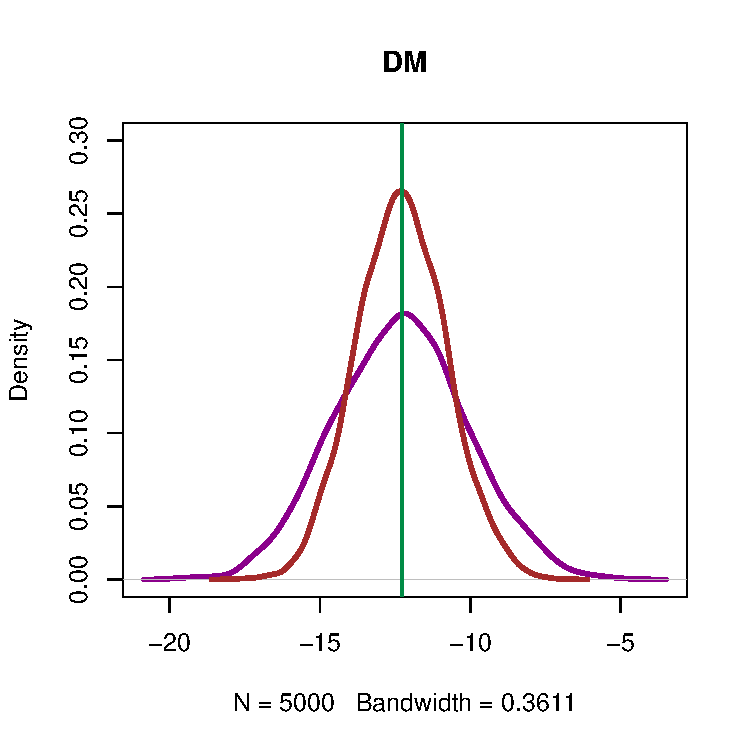
\includegraphics[width=\maxwidth]{figure/minimal-unnamed-chunk-5-1} 

}



\end{knitrout}

\begin{knitrout}
\definecolor{shadecolor}{rgb}{0.969, 0.969, 0.969}\color{fgcolor}\begin{kframe}
\begin{alltt}
\hlkwd{apply}\hlstd{(reps,} \hlkwc{MARGIN} \hlstd{=} \hlnum{1}\hlstd{,} \hlkwc{FUN} \hlstd{= mean)}
\end{alltt}
\begin{verbatim}
##        DM       DiD 
## -12.30131 -12.28649
\end{verbatim}
\begin{alltt}
\hlkwd{apply}\hlstd{(reps,} \hlkwc{MARGIN} \hlstd{=} \hlnum{1}\hlstd{,} \hlkwc{FUN} \hlstd{= sd)}
\end{alltt}
\begin{verbatim}
##       DM      DiD 
## 2.204130 1.489207
\end{verbatim}
\end{kframe}
\end{knitrout}

What can we say about the difference between these estimators? Is one of them "better"? If so, how so?

Our simulation shows the unbiasedness of the DiD estimator. 

In terms of precision, we saw in lecture that the DiD estimator may be more precise, but that this is true only when the pre-treatment value of the outcome strongly predicts potential outcomes. Formally, 

$$ Cov(Y_i(0), X_i) + Cov(Y_i(1), X_i) > Var(X_i) $$

What are the values for these elements in our example?
\begin{knitrout}
\definecolor{shadecolor}{rgb}{0.969, 0.969, 0.969}\color{fgcolor}\begin{kframe}
\begin{alltt}
\hlkwd{var}\hlstd{(conflict_pre)}
\end{alltt}
\begin{verbatim}
## [1] 15.4925
\end{verbatim}
\begin{alltt}
\hlkwd{cov}\hlstd{(y_i1, conflict_pre)}
\end{alltt}
\begin{verbatim}
## [1] 43.16722
\end{verbatim}
\begin{alltt}
\hlkwd{cov}\hlstd{(y_i0, conflict_pre)}
\end{alltt}
\begin{verbatim}
## [1] 38.70579
\end{verbatim}
\begin{alltt}
\hlkwd{cov}\hlstd{(y_i1, conflict_pre)} \hlopt{+} \hlkwd{cov}\hlstd{(y_i0, conflict_pre)} \hlopt{>}
    \hlkwd{var}\hlstd{(conflict_pre)}
\end{alltt}
\begin{verbatim}
## [1] TRUE
\end{verbatim}
\end{kframe}
\end{knitrout}

\textbf{In your next problem set:} How can we modify the simulation to show that the gains in precision depend on whether the pre-treatment value of the outcome strongly predicts potential outcomes?

\clearpage
\section*{Randomization inference with covariates (Rosenbaum 2002)}

We first create a DGP with a set of covariates that are predictive of the potential outcomes. 
\begin{knitrout}
\definecolor{shadecolor}{rgb}{0.969, 0.969, 0.969}\color{fgcolor}\begin{kframe}
\begin{alltt}
\hlkwd{library}\hlstd{(mvtnorm)}

\hlcom{# DGP}
\hlstd{sigma} \hlkwb{<-} \hlkwd{matrix}\hlstd{(}\hlnum{1}\hlstd{,} \hlnum{5}\hlstd{,} \hlnum{5}\hlstd{)}
\hlkwd{diag}\hlstd{(sigma)} \hlkwb{<-} \hlnum{2}
\hlstd{data} \hlkwb{<-} \hlkwd{as.data.frame}\hlstd{(}\hlkwd{rmvnorm}\hlstd{(}\hlkwc{n} \hlstd{=} \hlnum{300}\hlstd{,} \hlkwc{mean} \hlstd{=} \hlkwd{rep}\hlstd{(}\hlnum{0}\hlstd{,}
    \hlnum{5}\hlstd{),} \hlkwc{sigma} \hlstd{= sigma))}
\hlkwd{names}\hlstd{(data)[}\hlnum{1}\hlstd{]} \hlkwb{<-} \hlstr{"r0"}
\hlstd{data}\hlopt{$}\hlstd{r1} \hlkwb{<-} \hlstd{data}\hlopt{$}\hlstd{r0} \hlopt{+} \hlkwd{rnorm}\hlstd{(}\hlnum{300}\hlstd{,} \hlnum{0.2}\hlstd{,} \hlnum{1}\hlstd{)}  \hlcom{# ATE = .2}
\hlstd{data}\hlopt{$}\hlstd{Z} \hlkwb{<-} \hlkwd{rbinom}\hlstd{(}\hlnum{300}\hlstd{,} \hlnum{1}\hlstd{,} \hlnum{0.5}\hlstd{)}
\hlstd{data}\hlopt{$}\hlstd{yobs} \hlkwb{<-} \hlkwd{ifelse}\hlstd{(data}\hlopt{$}\hlstd{Z} \hlopt{==} \hlnum{1}\hlstd{, data}\hlopt{$}\hlstd{r1, data}\hlopt{$}\hlstd{r0)}
\end{alltt}
\end{kframe}
\end{knitrout}

We define a function that will produce residuals, $\epsilon(Y (0), X) = e$. The function could be pretty much anything as long as it was \textbf{definded before the treatment}. Here we will just a regression of Y (which is also Y(0) under the sharp null) on our four covariates. 

\begin{knitrout}
\definecolor{shadecolor}{rgb}{0.969, 0.969, 0.969}\color{fgcolor}\begin{kframe}
\begin{alltt}
\hlstd{e} \hlkwb{<-} \hlkwd{lm}\hlstd{(data}\hlopt{$}\hlstd{yobs} \hlopt{~} \hlstd{data}\hlopt{$}\hlstd{V2} \hlopt{+} \hlstd{data}\hlopt{$}\hlstd{V3} \hlopt{+} \hlstd{data}\hlopt{$}\hlstd{V4} \hlopt{+}
    \hlstd{data}\hlopt{$}\hlstd{V5)}\hlopt{$}\hlstd{residuals}
\end{alltt}
\end{kframe}
\end{knitrout}

We store the residuals from the regression, which will serve as our outcome variable.

We now get our test statistic of interest. Here we will just get the difference of means (remember regression is algebraically equivalent).

\begin{knitrout}
\definecolor{shadecolor}{rgb}{0.969, 0.969, 0.969}\color{fgcolor}\begin{kframe}
\begin{alltt}
\hlstd{Tstat} \hlkwb{<-} \hlkwd{mean}\hlstd{(e[data}\hlopt{$}\hlstd{Z} \hlopt{==} \hlnum{1}\hlstd{])} \hlopt{-} \hlkwd{mean}\hlstd{(e[data}\hlopt{$}\hlstd{Z} \hlopt{==}
    \hlnum{0}\hlstd{])}
\hlstd{Tstat}
\end{alltt}
\begin{verbatim}
## [1] 0.2078875
\end{verbatim}
\end{kframe}
\end{knitrout}

Now we need the randomization distribution. First we get the randomization matrix:
\begin{knitrout}
\definecolor{shadecolor}{rgb}{0.969, 0.969, 0.969}\color{fgcolor}\begin{kframe}
\begin{alltt}
\hlstd{fakeZ} \hlkwb{<-} \hlkwd{matrix}\hlstd{(}\hlnum{NA}\hlstd{,} \hlnum{300}\hlstd{,} \hlnum{10000}\hlstd{)}
\hlkwa{for} \hlstd{(i} \hlkwa{in} \hlnum{1}\hlopt{:}\hlnum{10000}\hlstd{) \{}
    \hlstd{fakeZ[, i]} \hlkwb{<-} \hlkwd{sample}\hlstd{(data}\hlopt{$}\hlstd{Z,} \hlnum{300}\hlstd{,} \hlkwc{replace} \hlstd{= F)}
\hlstd{\}}
\end{alltt}
\end{kframe}
\end{knitrout}

And get a tstatistic for each random treatment vector.
\begin{knitrout}
\definecolor{shadecolor}{rgb}{0.969, 0.969, 0.969}\color{fgcolor}\begin{kframe}
\begin{alltt}
\hlcom{# function}
\hlstd{DM} \hlkwb{<-} \hlkwa{function}\hlstd{(}\hlkwc{e}\hlstd{,} \hlkwc{z}\hlstd{) \{}
    \hlkwd{return}\hlstd{(}\hlkwd{mean}\hlstd{(e[z} \hlopt{==} \hlnum{1}\hlstd{])} \hlopt{-} \hlkwd{mean}\hlstd{(e[z} \hlopt{==} \hlnum{0}\hlstd{]))}
\hlstd{\}}

\hlstd{fakeTstats} \hlkwb{<-} \hlkwd{apply}\hlstd{(fakeZ,} \hlnum{2}\hlstd{, DM,} \hlkwc{e} \hlstd{= e)}
\end{alltt}
\end{kframe}
\end{knitrout}

\begin{knitrout}
\definecolor{shadecolor}{rgb}{0.969, 0.969, 0.969}\color{fgcolor}\begin{kframe}
\begin{alltt}
\hlkwd{hist}\hlstd{(fakeTstats,} \hlkwc{col} \hlstd{=} \hlstr{"grey80"}\hlstd{)}
\hlkwd{abline}\hlstd{(}\hlkwc{v} \hlstd{= Tstat,} \hlkwc{col} \hlstd{=} \hlstr{"springgreen4"}\hlstd{,} \hlkwc{lwd} \hlstd{=} \hlnum{4}\hlstd{)}
\end{alltt}
\end{kframe}

{\centering 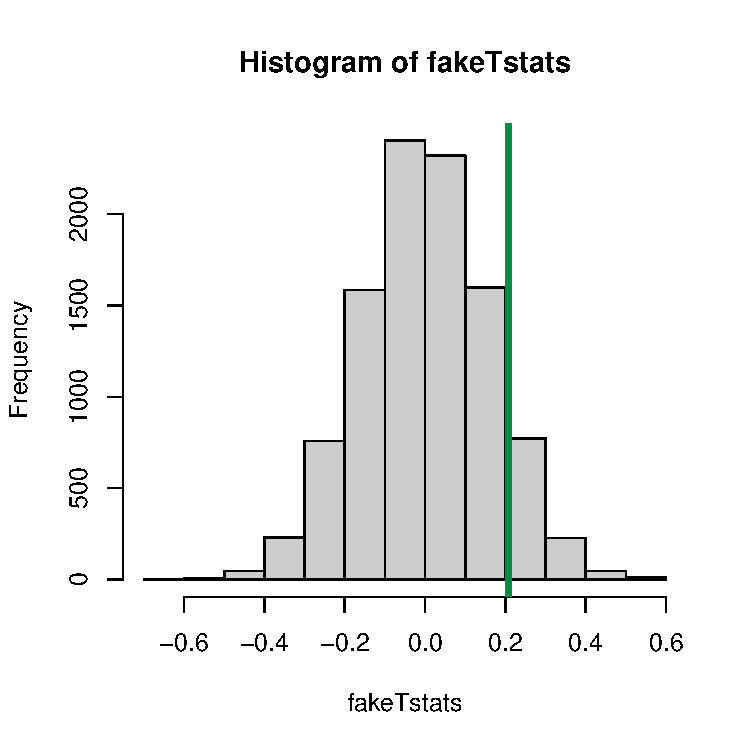
\includegraphics[width=\maxwidth]{figure/minimal-unnamed-chunk-13-1} 

}



\end{knitrout}

Finally, we calculate the p-value.
\begin{knitrout}
\definecolor{shadecolor}{rgb}{0.969, 0.969, 0.969}\color{fgcolor}\begin{kframe}
\begin{alltt}
\hlstd{pvalue} \hlkwb{<-} \hlkwd{sum}\hlstd{(}\hlkwd{abs}\hlstd{(fakeTstats)} \hlopt{>=} \hlstd{Tstat)}\hlopt{/}\hlnum{10000}
\hlstd{pvalue}
\end{alltt}
\begin{verbatim}
## [1] 0.192
\end{verbatim}
\end{kframe}
\end{knitrout}


\clearpage

\section*{Clustering}

DGP
\begin{knitrout}
\definecolor{shadecolor}{rgb}{0.969, 0.969, 0.969}\color{fgcolor}\begin{kframe}
\begin{alltt}
\hlstd{m} \hlkwb{<-} \hlnum{80}  \hlcom{# cluster size}
\hlstd{C} \hlkwb{<-} \hlnum{100}  \hlcom{# nr of clusters}
\hlstd{N} \hlkwb{<-} \hlstd{m} \hlopt{*} \hlstd{C}
\hlstd{cl} \hlkwb{<-} \hlkwd{rep}\hlstd{(}\hlnum{1}\hlopt{:}\hlstd{C,} \hlkwc{each} \hlstd{= m)}

\hlstd{y_0} \hlkwb{<-} \hlkwd{c}\hlstd{(}\hlkwd{rnorm}\hlstd{(N}\hlopt{/}\hlnum{8}\hlstd{,} \hlnum{0}\hlstd{,} \hlnum{2}\hlstd{),} \hlkwd{rnorm}\hlstd{(N}\hlopt{/}\hlnum{4}\hlstd{,} \hlnum{3}\hlstd{,} \hlnum{2}\hlstd{),} \hlkwd{rnorm}\hlstd{(N}\hlopt{/}\hlnum{4}\hlstd{,}
    \hlnum{5}\hlstd{,} \hlnum{1}\hlstd{),} \hlkwd{rnorm}\hlstd{(N}\hlopt{/}\hlnum{4}\hlstd{,} \hlnum{7}\hlstd{,} \hlnum{1}\hlstd{),} \hlkwd{rnorm}\hlstd{(N}\hlopt{/}\hlnum{8}\hlstd{,} \hlnum{8}\hlstd{,} \hlnum{2}\hlstd{))}
\hlstd{y_1} \hlkwb{<-} \hlstd{y_0} \hlopt{+} \hlkwd{rnorm}\hlstd{(N,} \hlnum{3}\hlstd{,} \hlnum{1}\hlstd{)}
\end{alltt}
\end{kframe}
\end{knitrout}

What is the average causal effect?
\begin{knitrout}
\definecolor{shadecolor}{rgb}{0.969, 0.969, 0.969}\color{fgcolor}\begin{kframe}
\begin{alltt}
\hlstd{ACE} \hlkwb{<-} \hlkwd{mean}\hlstd{(y_1)} \hlopt{-} \hlkwd{mean}\hlstd{(y_0)}
\hlstd{ACE}
\end{alltt}
\begin{verbatim}
## [1] 3.000605
\end{verbatim}
\end{kframe}
\end{knitrout}

We will assign 4000 units to treatment and 4000 to control

\begin{knitrout}
\definecolor{shadecolor}{rgb}{0.969, 0.969, 0.969}\color{fgcolor}\begin{kframe}
\begin{alltt}
\hlstd{simulation} \hlkwb{<-} \hlkwa{function}\hlstd{() \{}

    \hlcom{# simple random sampling}
    \hlstd{simple_random} \hlkwb{<-} \hlkwd{sample}\hlstd{(}\hlkwd{c}\hlstd{(}\hlkwd{rep}\hlstd{(}\hlnum{1}\hlstd{, N}\hlopt{/}\hlnum{2}\hlstd{),} \hlkwd{rep}\hlstd{(}\hlnum{0}\hlstd{,}
        \hlstd{N}\hlopt{/}\hlnum{2}\hlstd{)), N,} \hlkwc{replace} \hlstd{= F)}

    \hlcom{# cluster random sampling}
    \hlstd{clusters_treat} \hlkwb{<-} \hlkwd{sample}\hlstd{(}\hlnum{1}\hlopt{:}\hlstd{C, C}\hlopt{/}\hlnum{2}\hlstd{,} \hlkwc{replace} \hlstd{=} \hlnum{FALSE}\hlstd{)}
    \hlstd{g} \hlkwb{<-} \hlkwa{function}\hlstd{(}\hlkwc{x}\hlstd{) \{}
        \hlkwd{sum}\hlstd{(x} \hlopt{==} \hlstd{clusters_treat)}
    \hlstd{\}}
    \hlstd{cluster_random} \hlkwb{<-} \hlkwd{unlist}\hlstd{(}\hlkwd{lapply}\hlstd{(cl,} \hlkwc{FUN} \hlstd{= g))}

    \hlcom{# diff in means simple random assignment}
    \hlstd{dm_sr} \hlkwb{<-} \hlkwd{mean}\hlstd{(y_1[simple_random} \hlopt{==} \hlnum{1}\hlstd{])} \hlopt{-} \hlkwd{mean}\hlstd{(y_0[simple_random} \hlopt{==}
        \hlnum{0}\hlstd{])}

    \hlcom{# diff in means cluster assignment, individual}
    \hlstd{dm_cl} \hlkwb{<-} \hlkwd{mean}\hlstd{(y_1[cluster_random} \hlopt{==} \hlnum{1}\hlstd{])} \hlopt{-}
        \hlkwd{mean}\hlstd{(y_0[cluster_random} \hlopt{==} \hlnum{0}\hlstd{])}

    \hlcom{# diff in means cluster assignment, cluster}
    \hlcom{# means}
    \hlstd{cl_treat} \hlkwb{<-} \hlkwd{unlist}\hlstd{(}\hlkwd{lapply}\hlstd{(clusters_treat,}
        \hlkwc{FUN} \hlstd{=} \hlkwa{function}\hlstd{(}\hlkwc{x}\hlstd{)} \hlkwd{mean}\hlstd{(y_1[cl} \hlopt{==} \hlstd{x])))}
    \hlstd{cl_control} \hlkwb{<-} \hlkwd{unlist}\hlstd{(}\hlkwd{lapply}\hlstd{(}\hlkwd{as.vector}\hlstd{(}\hlnum{1}\hlopt{:}\hlstd{C)[}\hlopt{-}\hlstd{(clusters_treat)],}
        \hlkwc{FUN} \hlstd{=} \hlkwa{function}\hlstd{(}\hlkwc{x}\hlstd{)} \hlkwd{mean}\hlstd{(y_0[cl} \hlopt{==} \hlstd{x])))}
    \hlstd{dm_cl_cl} \hlkwb{<-} \hlkwd{mean}\hlstd{(cl_treat)} \hlopt{-} \hlkwd{mean}\hlstd{(cl_control)}

    \hlkwd{return}\hlstd{(}\hlkwd{c}\hlstd{(dm_sr, dm_cl, dm_cl_cl))}

\hlstd{\}}
\end{alltt}
\end{kframe}
\end{knitrout}


\begin{knitrout}
\definecolor{shadecolor}{rgb}{0.969, 0.969, 0.969}\color{fgcolor}\begin{kframe}
\begin{alltt}
\hlkwd{simulation}\hlstd{()}
\end{alltt}
\begin{verbatim}
## [1] 2.907437 2.732269 2.732269
\end{verbatim}
\begin{alltt}
\hlstd{sims} \hlkwb{<-} \hlkwd{replicate}\hlstd{(}\hlnum{10000}\hlstd{,} \hlkwd{simulation}\hlstd{())}
\end{alltt}
\end{kframe}
\end{knitrout}

How do we expect the results to look like?


\begin{knitrout}
\definecolor{shadecolor}{rgb}{0.969, 0.969, 0.969}\color{fgcolor}\begin{kframe}
\begin{alltt}
\hlkwd{plot}\hlstd{(}\hlkwd{density}\hlstd{(sims[}\hlnum{1}\hlstd{, ]),} \hlkwc{col} \hlstd{=} \hlstr{"red"}\hlstd{,} \hlkwc{lwd} \hlstd{=} \hlnum{3}\hlstd{,}
    \hlkwc{xlim} \hlstd{=} \hlkwd{c}\hlstd{(}\hlkwd{min}\hlstd{(sims),} \hlkwd{max}\hlstd{(sims)))}
\hlkwd{abline}\hlstd{(}\hlkwc{v} \hlstd{= ACE,} \hlkwc{col} \hlstd{=} \hlstr{"grey"}\hlstd{,} \hlkwc{lwd} \hlstd{=} \hlnum{3}\hlstd{)}
\end{alltt}
\end{kframe}

{\centering 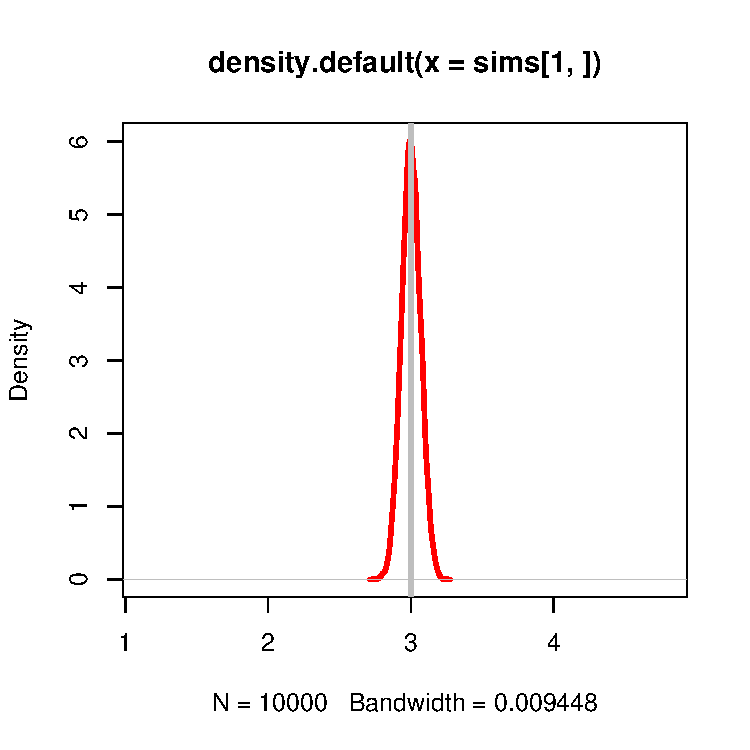
\includegraphics[width=\maxwidth]{figure/minimal-unnamed-chunk-19-1} 

}



\end{knitrout}

\begin{knitrout}
\definecolor{shadecolor}{rgb}{0.969, 0.969, 0.969}\color{fgcolor}\begin{kframe}
\begin{alltt}
\hlkwd{plot}\hlstd{(}\hlkwd{density}\hlstd{(sims[}\hlnum{1}\hlstd{, ]),} \hlkwc{col} \hlstd{=} \hlstr{"red"}\hlstd{,} \hlkwc{lwd} \hlstd{=} \hlnum{3}\hlstd{,}
    \hlkwc{xlim} \hlstd{=} \hlkwd{c}\hlstd{(}\hlkwd{min}\hlstd{(sims),} \hlkwd{max}\hlstd{(sims)))}
\hlkwd{abline}\hlstd{(}\hlkwc{v} \hlstd{= ACE,} \hlkwc{col} \hlstd{=} \hlstr{"grey"}\hlstd{,} \hlkwc{lwd} \hlstd{=} \hlnum{3}\hlstd{)}
\hlkwd{lines}\hlstd{(}\hlkwd{density}\hlstd{(sims[}\hlnum{2}\hlstd{, ]),} \hlkwc{col} \hlstd{=} \hlstr{"slateblue"}\hlstd{,} \hlkwc{lwd} \hlstd{=} \hlnum{3}\hlstd{)}
\hlkwd{lines}\hlstd{(}\hlkwd{density}\hlstd{(sims[}\hlnum{3}\hlstd{, ]),} \hlkwc{col} \hlstd{=} \hlstr{"deepskyblue"}\hlstd{,}
    \hlkwc{lwd} \hlstd{=} \hlnum{3}\hlstd{,} \hlkwc{lty} \hlstd{=} \hlnum{3}\hlstd{)}
\end{alltt}
\end{kframe}

{\centering 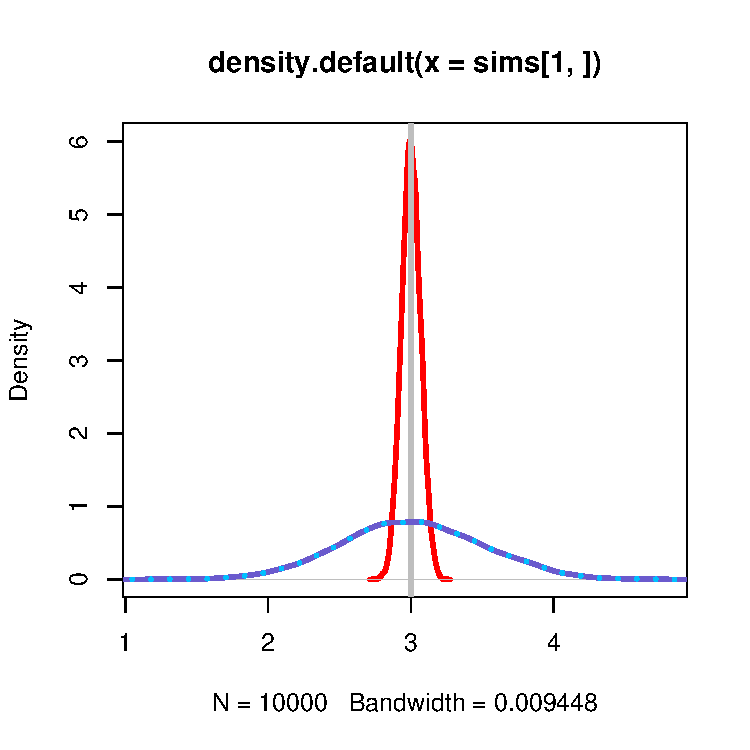
\includegraphics[width=\maxwidth]{figure/minimal-unnamed-chunk-20-1} 

}



\end{knitrout}

\begin{knitrout}
\definecolor{shadecolor}{rgb}{0.969, 0.969, 0.969}\color{fgcolor}\begin{kframe}
\begin{alltt}
\hlkwd{apply}\hlstd{(sims,} \hlkwc{MARGIN} \hlstd{=} \hlnum{1}\hlstd{,} \hlkwc{FUN} \hlstd{= mean)}
\end{alltt}
\begin{verbatim}
## [1] 3.001028 3.008015 3.008015
\end{verbatim}
\begin{alltt}
\hlkwd{apply}\hlstd{(sims,} \hlkwc{MARGIN} \hlstd{=} \hlnum{1}\hlstd{,} \hlkwc{FUN} \hlstd{= sd)}
\end{alltt}
\begin{verbatim}
## [1] 0.0662361 0.4962054 0.4962054
\end{verbatim}
\end{kframe}
\end{knitrout}


\clearpage
\section*{OLS and Heteroscedasticity}

\subsection*{The problem:}
Setup
\begin{knitrout}
\definecolor{shadecolor}{rgb}{0.969, 0.969, 0.969}\color{fgcolor}\begin{kframe}
\begin{alltt}
\hlstd{y_0} \hlkwb{<-} \hlkwd{rnorm}\hlstd{(}\hlnum{100}\hlstd{,} \hlnum{0}\hlstd{,} \hlnum{1}\hlstd{)}
\hlstd{y_1} \hlkwb{<-} \hlstd{y_0} \hlopt{+} \hlkwd{rnorm}\hlstd{(}\hlnum{100}\hlstd{,} \hlnum{2}\hlstd{,} \hlnum{10}\hlstd{)}

\hlkwd{sd}\hlstd{(y_0)}
\end{alltt}
\begin{verbatim}
## [1] 0.9669063
\end{verbatim}
\begin{alltt}
\hlkwd{sd}\hlstd{(y_1)}
\end{alltt}
\begin{verbatim}
## [1] 9.895268
\end{verbatim}
\begin{alltt}
\hlstd{treat} \hlkwb{<-} \hlkwd{rbinom}\hlstd{(}\hlnum{100}\hlstd{,} \hlnum{1}\hlstd{,} \hlnum{0.5}\hlstd{)}
\hlstd{Y} \hlkwb{<-} \hlkwd{ifelse}\hlstd{(treat} \hlopt{==} \hlnum{1}\hlstd{, y_1, y_0)}
\end{alltt}
\end{kframe}
\end{knitrout}

\begin{knitrout}
\definecolor{shadecolor}{rgb}{0.969, 0.969, 0.969}\color{fgcolor}\begin{kframe}
\begin{alltt}
\hlkwd{source}\hlstd{(}\hlstr{"~/Dropbox/Resources/r_functions/t_test.R"}\hlstd{)}
\hlkwd{ttest}\hlstd{(Y, treat)}
\end{alltt}
\begin{verbatim}
##       Mean 1       Mean 0   Difference 
##   0.86621324  -0.02155845   0.88777170 
##      SE_Diff       t-stat            N 
##   1.32144219   0.67182031 100.00000000 
##           df      p-value 
##  44.68175096   0.50515711
\end{verbatim}
\begin{alltt}
\hlkwd{summary}\hlstd{(}\hlkwd{lm}\hlstd{(Y} \hlopt{~} \hlstd{treat))}
\end{alltt}
\begin{verbatim}
## 
## Call:
## lm(formula = Y ~ treat)
## 
## Residuals:
##      Min       1Q   Median       3Q      Max 
## -22.5782  -1.0053  -0.0571   1.0120  23.4088 
## 
## Coefficients:
##             Estimate Std. Error t value
## (Intercept) -0.02156    0.80245  -0.027
## treat        0.88777    1.19622   0.742
##             Pr(>|t|)
## (Intercept)    0.979
## treat          0.460
## 
## Residual standard error: 5.951 on 98 degrees of freedom
## Multiple R-squared:  0.005589,	Adjusted R-squared:  -0.004558 
## F-statistic: 0.5508 on 1 and 98 DF,  p-value: 0.4598
\end{verbatim}
\end{kframe}
\end{knitrout}


As you have shown in your problem sets, it will often be the case in experiments that 
$$E(\epsilon|T) \not= \sigma^2$$ 
Indeed,
$$E(\epsilon_i|T_i=1)=Var(Y_i(1))$$
$$E(\epsilon_i|T_i=0)=Var(Y_i(0))$$
which are only equal when $$Var(Y_i(1))=Var(Y_i(0))$$


Back to section 4: \textbf{How do we calculate $SE(\hat{\beta})$ when we assume homoskedasticity?}

\begin{knitrout}
\definecolor{shadecolor}{rgb}{0.969, 0.969, 0.969}\color{fgcolor}\begin{kframe}
\begin{alltt}
\hlcom{# The first thing we will need here is to}
\hlcom{# build the matrix for X}
\hlstd{X} \hlkwb{<-} \hlkwd{cbind}\hlstd{(}\hlnum{1}\hlstd{, treat)}

\hlcom{# getting the betas}
\hlstd{betas} \hlkwb{<-} \hlkwd{solve}\hlstd{(}\hlkwd{t}\hlstd{(X)} \hlopt \hlstd{X)} \hlopt \hlkwd{t}\hlstd{(X)} \hlopt \hlstd{Y}

\hlcom{# and the residuals}
\hlstd{e} \hlkwb{<-} \hlstd{Y} \hlopt{-} \hlstd{X} \hlopt \hlstd{betas}

\hlcom{# and now we want the estimated sigma squared}
\hlstd{hat_sigma2} \hlkwb{<-} \hlkwd{sum}\hlstd{(}\hlkwd{t}\hlstd{(e)} \hlopt \hlstd{e)}\hlopt{/}\hlstd{(}\hlkwd{nrow}\hlstd{(X)} \hlopt{-} \hlkwd{length}\hlstd{(betas))}

\hlcom{# and we can find estimated standard errors}
\hlcom{# from $\textbackslash{}hat\{\textbackslash{}sigma^2\}(X'X)^\{-1\}$.}
\hlstd{var_hat_beta} \hlkwb{<-} \hlstd{hat_sigma2} \hlopt{*} \hlkwd{solve}\hlstd{((}\hlkwd{t}\hlstd{(X)} \hlopt \hlstd{X))}  \hlcom{# Why do we use * instead of %*% here?}

\hlcom{# and get the SEs for our betas}
\hlstd{se_hat_beta} \hlkwb{<-} \hlkwd{sqrt}\hlstd{(}\hlkwd{diag}\hlstd{(var_hat_beta))}
\hlstd{se_hat_beta}
\end{alltt}
\begin{verbatim}
##               treat 
## 0.8024517 1.1962244
\end{verbatim}
\end{kframe}
\end{knitrout}

\subsection*{The White-Huber correction}

$$\hat{cov}(\hat{\beta})=(X'X)^{-1}(X'\hat{G}X)(X'X)^{-1}$$

The shortcut
\begin{knitrout}
\definecolor{shadecolor}{rgb}{0.969, 0.969, 0.969}\color{fgcolor}\begin{kframe}
\begin{alltt}
\hlkwd{library}\hlstd{(sandwich)}
\hlstd{fit} \hlkwb{<-} \hlkwd{lm}\hlstd{(Y} \hlopt{~} \hlstd{treat)}
\hlkwd{sqrt}\hlstd{(}\hlkwd{vcovHC}\hlstd{(fit,} \hlkwc{type} \hlstd{=} \hlstr{"HC0"}\hlstd{)[}\hlnum{2}\hlstd{,} \hlnum{2}\hlstd{])}
\end{alltt}
\begin{verbatim}
## [1] 1.306698
\end{verbatim}
\end{kframe}
\end{knitrout}


Let's go through what happens under the hood:

First we need the ``bread'': $(X'X)$
\begin{knitrout}
\definecolor{shadecolor}{rgb}{0.969, 0.969, 0.969}\color{fgcolor}\begin{kframe}
\begin{alltt}
\hlstd{bread} \hlkwb{<-} \hlkwd{solve}\hlstd{(}\hlkwd{t}\hlstd{(X)} \hlopt \hlstd{X)}
\end{alltt}
\end{kframe}
\end{knitrout}

And ``butter'':
\begin{knitrout}
\definecolor{shadecolor}{rgb}{0.969, 0.969, 0.969}\color{fgcolor}\begin{kframe}
\begin{alltt}
\hlstd{Ghat} \hlkwb{<-} \hlkwd{diag}\hlstd{(fit}\hlopt{$}\hlstd{residuals)}\hlopt{^}\hlnum{2}

\hlstd{butter} \hlkwb{<-} \hlkwd{t}\hlstd{(X)} \hlopt \hlstd{Ghat} \hlopt \hlstd{X}
\end{alltt}
\end{kframe}
\end{knitrout}


\begin{knitrout}
\definecolor{shadecolor}{rgb}{0.969, 0.969, 0.969}\color{fgcolor}\begin{kframe}
\begin{alltt}
\hlstd{EHW} \hlkwb{<-} \hlstd{bread} \hlopt \hlstd{butter} \hlopt \hlstd{bread}
\end{alltt}
\end{kframe}
\end{knitrout}

What elements from this matrix do we need?
\begin{knitrout}
\definecolor{shadecolor}{rgb}{0.969, 0.969, 0.969}\color{fgcolor}\begin{kframe}
\begin{alltt}
\hlkwd{sqrt}\hlstd{(EHW[}\hlnum{2}\hlstd{,} \hlnum{2}\hlstd{])}
\end{alltt}
\begin{verbatim}
## [1] 1.306698
\end{verbatim}
\end{kframe}
\end{knitrout}

Let's compare this to the results from the t-test:
\begin{knitrout}
\definecolor{shadecolor}{rgb}{0.969, 0.969, 0.969}\color{fgcolor}\begin{kframe}
\begin{alltt}
\hlkwd{ttest}\hlstd{(Y, treat)}
\end{alltt}
\begin{verbatim}
##       Mean 1       Mean 0   Difference 
##   0.86621324  -0.02155845   0.88777170 
##      SE_Diff       t-stat            N 
##   1.32144219   0.67182031 100.00000000 
##           df      p-value 
##  44.68175096   0.50515711
\end{verbatim}
\end{kframe}
\end{knitrout}

\end{document}
